% Chapter 3: Design and Architecture


\chapter{Design and Architecture}


\section{Global System Architecture}

\subsection{Overview}

The financial data surveillance system is designed as a distributed, event-driven architecture composed of several interconnected microservices. This architecture ensures scalability, resilience, and maintainability, which are critical for real-time financial applications.

\begin{figure}[H]
    \centering
    % Placeholder for the general architecture diagram
    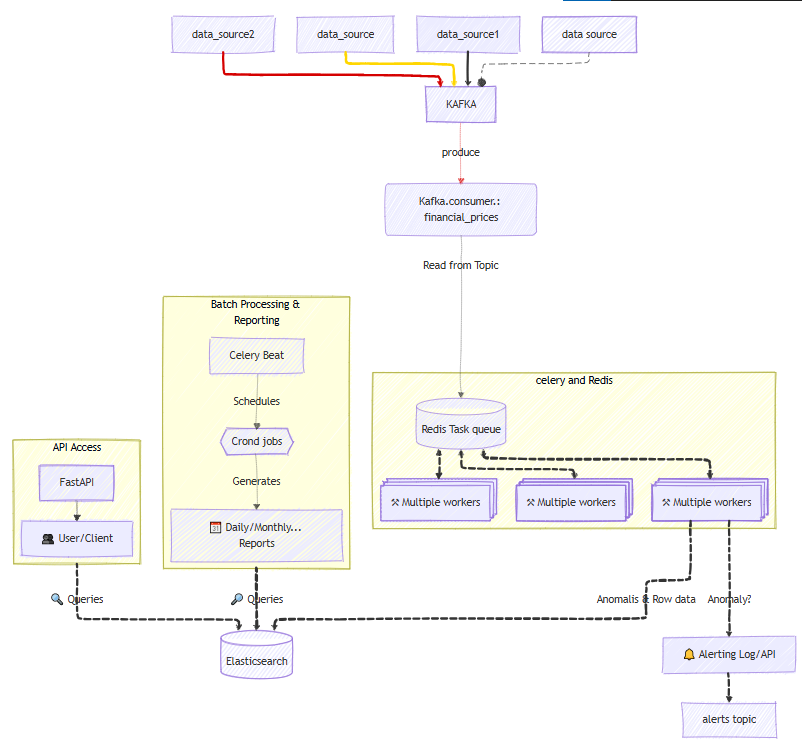
\includegraphics[width=\textwidth]{figures/global.png}
    % \fbox{\parbox[c][10cm][c]{\textwidth}{\centering Placeholder for General Architecture Diagram (e.g., using TikZ or an imported image)}}
    % \caption{General System Architecture}
    % \label{fig:general_architecture}
\end{figure}

\textbf{Main Data Flow:}
\begin{enumerate}
    \item \textbf{Data Ingestion}: Simulated financial data (e.g., TSLA stock prices) is generated and published to an Apache Kafka topic.
    \item \textbf{Real-time Processing}: Kafka consumers read data streams, and Celery workers process these messages asynchronously to detect anomalies using the Z-score algorithm. Redis is used for storing sliding windows of recent data for calculations.
    \item \textbf{Anomaly Storage}: Detected anomalies are indexed and stored in Elasticsearch for historical analysis and querying.
    \item \textbf{API and Reporting}: A FastAPI application provides RESTful endpoints for querying anomalies, generating reports (PDF, CSV), and managing alerts. Alerts are also published to separate Kafka topics for consumption by notification services.
\end{enumerate}

\textbf{Components and Their Interactions:}
\begin{itemize}
    \item \textbf{Data Generator}: Produces simulated stock price data.
    \item \textbf{Kafka Cluster}: Acts as the central message bus for data streams and alerts.
    \item \textbf{Celery Workers}: Perform asynchronous anomaly detection tasks.
    \item \textbf{Redis}: Provides fast, in-memory storage for sliding windows.
    \item \textbf{Elasticsearch Cluster}: Stores and indexes detected anomalies for long-term analysis.
    \item \textbf{FastAPI Application}: Exposes system functionalities through a REST API.
    \item \textbf{Reporting Module}: Generates analytical reports.
    \item \textbf{Alerting System}: Manages and dispatches alerts.
\end{itemize}

\subsection{Architectural Pattern}

\subsubsection{Microservices Architecture}

The choice of a microservices architecture is justified by:
\begin{itemize}
    \item \textbf{Scalability}: Individual services can be scaled independently based on demand (e.g., scaling Celery workers during high data load).
    \item \textbf{Resilience}: Failure in one service does not necessarily bring down the entire system. For instance, if the reporting service fails, data ingestion and anomaly detection can continue.
    \item \textbf{Technology Diversity}: Different services can be implemented using the most suitable technology stack for their specific tasks.
    \item \textbf{Maintainability}: Smaller, focused services are easier to understand, develop, test, and maintain.
    \item \textbf{Independent Deployability}: Services can be deployed and updated independently, allowing for faster release cycles.
\end{itemize}

\subsubsection{Event-Driven Architecture (EDA)}

An event-driven architecture, primarily facilitated by Apache Kafka, offers several advantages:
\begin{itemize}
    \item \textbf{Decoupling}: Producers and consumers of data are decoupled. The data generator does not need to know about the anomaly detection workers, and vice-versa.
    \item \textbf{Asynchronous Processing}: Tasks like anomaly detection can be performed asynchronously, improving system responsiveness and throughput.
    \item \textbf{Scalability and Resilience}: Kafka itself is highly scalable and fault-tolerant, contributing to the overall system's robustness.
    \item \textbf{Real-time Capabilities}: EDA is well-suited for real-time applications where immediate response to events (like new price data) is crucial.
\end{itemize}

\subsubsection{Separation of Concerns}

Each layer and component in the architecture has a distinct responsibility:
\begin{itemize}
    \item \textbf{Data Collection Layer}: Focuses solely on ingesting and formatting raw data.
    \item \textbf{Processing Layer}: Handles the core logic of anomaly detection.
    \item \textbf{Storage Layer}: Manages persistent storage and indexing of anomalies.
    \item \textbf{API and Reporting Layer}: Provides interfaces for user interaction and data retrieval.
\end{itemize}
This separation simplifies development, testing, and maintenance.

\section{Technology Overview and Selection Rationale}

The implementation of this system relies on several key technologies, each chosen for specific capabilities they bring to the architecture. This section provides a focused explanation of each core technology and its role in the system.

\subsection{Apache Kafka}

\subsubsection{Overview}


\begin{wrapfigure}{l}{2.5cm}  % 'l' = left side, 2.5cm = width of the box
    \vspace{-10pt} % Adjust vertical spacing
    
\includegraphics[width=2.3cm]{figures/0_CuYxguE1vG7PLngW.png}
    \vspace{-10pt}
\end{wrapfigure}

Apache Kafka is a distributed event streaming platform used in our architecture for real-time data ingestion and message propagation. It provides a highly reliable, scalable system for publishing and subscribing to streams of records.



\subsubsection{Core Features}
\begin{itemize}
    \item \textbf{Distributed Architecture}: Kafka operates as a cluster of broker nodes, providing fault tolerance and load distribution.
    \item \textbf{Topic-Based Messaging}: Data streams are organized into topics that can be partitioned for parallel processing.
    \item \textbf{High Throughput}: Capable of handling millions of messages per second with minimal latency.
    \item \textbf{Persistent Storage}: Messages are persisted to disk with configurable retention periods.
    \item \textbf{Replication}: Data is replicated across multiple nodes to prevent data loss.
\end{itemize}

\subsubsection{Kafka Architecture}

\begin{figure}[H]
    \centering
    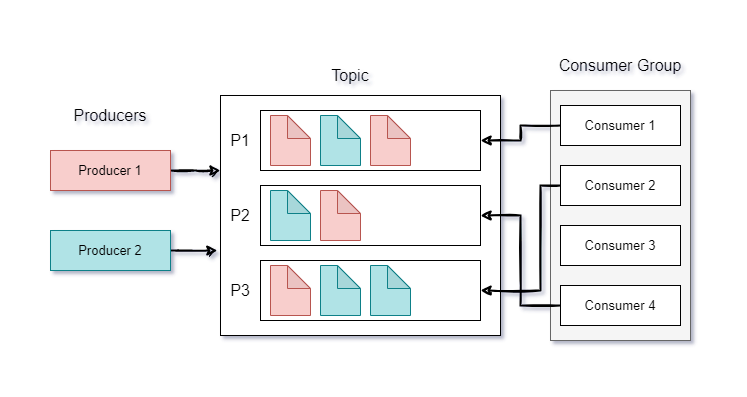
\includegraphics[width=0.75\textwidth]{figures/kafka.png}
    \caption{Kafka Architecture}
    \label{fig:kafka_architecture}
\end{figure}

\subsubsection{Role in Our System}
In our financial surveillance system, Kafka serves as:
\begin{itemize}
    \item The central data highway for stock price data streams
    \item A buffer system that decouples data producers from consumers
    \item A scalable mechanism for distributing data to multiple processing workers
    \item An event bus for propagating detected anomalies to notification services
\end{itemize}

\subsection{Redis}

\subsubsection{Overview}


\begin{wrapfigure}{l}{2.5cm}  % 'l' = left side, 2.5cm = width of the box
    \vspace{-10pt} % Adjust vertical spacing
    
\includegraphics[width=2.3cm]{figures/redis.png}
    \vspace{-10pt}
\end{wrapfigure}



Redis is an in-memory data structure store that we use both as a message broker for Celery and for maintaining sliding windows of recent stock data.

\subsubsection{Core Features}
\begin{itemize}
    \item \textbf{In-Memory Operation}: Extremely fast read/write operations with sub-millisecond latency.
    \item \textbf{Data Structures}: Supports various data structures like strings, hashes, lists, sets, and sorted sets.
    \item \textbf{Optional Persistence}: Can persist data to disk through snapshotting or append-only files.
    \item \textbf{Atomic Operations}: Supports transactions and Lua scripting for complex operations.
    \item \textbf{Pub/Sub Capabilities}: Native support for publish/subscribe messaging patterns.
\end{itemize}

\subsubsection{Role in Our System}
Redis performs two critical functions:
\begin{itemize}
    \item \textbf{Sliding Window Management}: Stores recent price data points for calculating moving statistics (mean, standard deviation) with extremely low latency.
    \item \textbf{Celery Broker}: Acts as the message broker for Celery, queuing anomaly detection tasks.
\end{itemize}

\subsection{Celery}

\subsubsection{Overview}


\begin{wrapfigure}{l}{2.5cm}  % 'l' = left side, 2.5cm = width of the box
    \vspace{-10pt} % Adjust vertical spacing
    
\includegraphics[width=2.3cm]{figures/Celery_logo.png}
    \vspace{-10pt}
\end{wrapfigure}



Celery is an asynchronous task queue/job system based on distributed message passing. It handles the background processing of anomaly detection in our architecture.

\subsubsection{Core Features}
\begin{itemize}
    \item \textbf{Asynchronous Task Execution}: Allows non-blocking execution of CPU-intensive or I/O-bound tasks.
    \item \textbf{Task Scheduling}: Supports both immediate and scheduled task execution.
    \item \textbf{Worker Pools}: Tasks can be distributed across multiple worker processes or machines.
    \item \textbf{Result Storage}: Task results can be stored and retrieved asynchronously.
    \item \textbf{Monitoring}: Tools like Flower provide real-time monitoring of task execution.
\end{itemize}

\subsubsection{Role in Our System}
Celery manages:
\begin{itemize}
    \item Asynchronous execution of anomaly detection algorithms
    \item Distribution of processing load across multiple worker instances
    \item Reliable task execution with automatic retries for failed tasks
\end{itemize}

\subsection{Elasticsearch}



\subsubsection{Overview}


\begin{wrapfigure}{l}{2.5cm}  % 'l' = left side, 2.5cm = width of the box
    \vspace{-10pt} % Adjust vertical spacing
    
\includegraphics[width=2.3cm]{figures/Elasticsearhc.png}
    \vspace{-10pt}
\end{wrapfigure}



Elasticsearch is a distributed, RESTful search and analytics engine used for storing and querying detected anomalies.

\subsubsection{Core Features}
\begin{itemize}
    \item \textbf{Document-Oriented}: Stores data as JSON documents with flexible schema.
    \item \textbf{Full-Text Search}: Powerful search capabilities with relevance scoring.
    \item \textbf{Analytics}: Built-in aggregation framework for data analytics.
    \item \textbf{Distributed Architecture}: Scales horizontally across multiple nodes.
    \item \textbf{Real-Time Operations}: Near real-time indexing and search capabilities.
\end{itemize}

\subsubsection{Role in Our System}
Elasticsearch serves as:
\begin{itemize}
    \item The persistent storage for detected anomalies
    \item A search engine for querying historical anomalies by various parameters (time range, symbol, severity)
    \item An analytics platform for trend analysis and reporting on anomalies
\end{itemize}

\subsection{FastAPI}

\subsubsection{Overview}

\begin{wrapfigure}{l}{2.5cm}  % 'l' = left side, 2.5cm = width of the box
    \vspace{-10pt} % Adjust vertical spacing
    
\includegraphics[width=2.3cm]{figures/FastAPI_logo.png}
    \vspace{-10pt}
\end{wrapfigure}


FastAPI is a modern, high-performance web framework for building APIs with Python, based on standard Python type hints.

\subsubsection{Core Features}
\begin{itemize}
    \item \textbf{Performance}: One of the fastest Python frameworks available, comparable to NodeJS and Go.
    \item \textbf{Automatic Documentation}: Generates interactive API documentation from code.
    \item \textbf{Data Validation}: Built-in request validation using Pydantic models.
    \item \textbf{Asynchronous Support}: Native support for async/await syntax.
    \item \textbf{Standards-Based}: Based on open standards like OpenAPI and JSON Schema.
\end{itemize}

\subsubsection{Role in Our System}
FastAPI provides:
\begin{itemize}
    \item RESTful endpoints for querying anomalies and generating reports
    \item A user-friendly API for interacting with the surveillance system
    \item Authentication and authorization for secure access to sensitive financial data
    \item Input validation for all API requests
\end{itemize}


\subsection{Docker}

\subsubsection{Overview}

\begin{wrapfigure}{l}{2.5cm}
    \vspace{-10pt}
    \includegraphics[width=2.3cm]{figures/docker.png}
    \vspace{-10pt}
\end{wrapfigure}

Docker is a platform for developing, shipping, and running applications in lightweight, portable containers. It enables consistent environments across development, testing, and production.

\subsubsection{Core Features}
\begin{itemize}
    \item \textbf{Containerization}: Packages applications and dependencies into isolated containers.
    \item \textbf{Portability}: Ensures applications run the same way on any system with Docker installed.
    \item \textbf{Resource Efficiency}: Containers share the host OS kernel, reducing overhead compared to virtual machines.
    \item \textbf{Rapid Deployment}: Containers can be started, stopped, and replicated quickly.
    \item \textbf{Ecosystem}: Rich tooling (Docker Compose, Docker Hub) and integration with CI/CD pipelines.
\end{itemize}

\subsubsection{Role in Our System}
Docker is used to:
\begin{itemize}
    \item Containerize all core services (Kafka, Redis, Elasticsearch, etc.) for reproducible deployments.
    \item Simplify orchestration and networking using Docker Compose.
    \item Enable easy scaling and management of microservices.
    \item Provide isolated, consistent environments for development and production.
\end{itemize}

\section{Detailed Components}

\subsection{Data Collection Layer}

\subsubsection{Data Generator}

A Python script simulates real-time stock price data for a specific symbol (e.g., TSLA). It generates data points with a timestamp, price, and volume, introducing occasional artificial anomalies to test the detection mechanism.
\begin{itemize}
    \item \textbf{Simulation Logic}: May include random walks with configurable volatility and drift, and occasional price spikes or drops.
    \item \textbf{Output Format}: JSON, to be easily consumed by Kafka.
\end{itemize}

\subsubsection{Kafka Producer}

Detected anomalies are stored in Elasticsearch for long-term persistence, efficient searching, and analytics.
\begin{itemize}
    \item \textbf{Index}: A dedicated index (e.g., \texttt{financial\_anomalies}) stores anomaly documents.
    \item \textbf{Document Structure}: Each anomaly document includes details like symbol, timestamp, price, Z-score, window mean, window standard deviation, and alert level.
\end{itemize}
\subsubsection{Message Format (JSON)}

A standardized JSON structure is used for messages published to Kafka:
\begin{minted}[fontsize=\footnotesize, frame=lines, label=JSON Message Format]{json}
{
  "timestamp": "2025-04-07 04:00:00",
  "symbol": "TSLA",
  "open": 218.04,
  "high": 222.23,
  "low": 214.80,
  "close": 215.50,
  "volume": 56581
}

\end{minted}

this diagram from different sources into the kafka topic \texttt{stock\_prices}.

\begin{figure}[H]
    
   
    % \hspace{-3cm}
    % \includegraphics[width=0.8\textwidth]{figures/class_diagram_data_model.png}
    \includegraphics[width=\textwidth]{figures/svgviewer-png-output.png}
    \caption{different sources into the kafka topic \texttt{stock\_prices}.}
    \label{fig:data_collection_layer_diagram}


\end{figure}




\subsection{Processing Layer}

\subsubsection{Kafka Consumer Script}

A dedicated Python script acts as the Kafka consumer, subscribing to the \texttt{stock\_prices} topic and bridging the gap between Kafka and Celery.
\begin{itemize}
    \item \textbf{Consumer Group}: The script joins a consumer group to enable parallel processing when multiple consumer instances are running.
    \item \textbf{Message Handling}: Upon receiving each message from the Kafka topic, the script immediately dispatches an anomaly detection task to the Celery queue.
    \item \textbf{Task Delegation}: For each data point consumed, the script calls the appropriate Celery task with the message payload as parameters.
    \item \textbf{Error Handling}: Implements retry logic and dead letter handling for failed message processing.
\end{itemize}

\subsubsection{Celery Workers}

Celery workers operate independently from Kafka, focusing solely on executing anomaly detection tasks queued by the consumer script.
\begin{itemize}
    \item \textbf{Task Definition}: Anomaly detection logic (Z-score calculation) is encapsulated in Celery tasks that receive stock price data as input parameters.
    \item \textbf{Broker}: Redis serves as the message broker between the Kafka consumer script and Celery workers.
    \item \textbf{Concurrency}: Multiple Celery workers can run concurrently to process the queued anomaly detection tasks.
    \item \textbf{Task Execution}: Workers retrieve tasks from the Redis queue, perform Z-score calculations, and store results in Elasticsearch if anomalies are detected.
\end{itemize}


this diagram will explain how the Kafka consumer script interacts with Celery workers and Redis(task queue).

\begin{figure}[H]
    \centering
    \includegraphics[width=\textwidth]{figures/image.png}
    \caption{Kafka Consumer and Celery Workers Interaction}
    \label{fig:consumer_celery_diagram}
\end{figure}

\paragraph{Scalability of Celery Workers}
Separating Celery workers from other system components enables horizontal scaling. Since Redis acts as a message broker and task queue, additional Celery workers can be added at any time to handle increased processing load. This architecture allows the system to efficiently distribute and process tasks in parallel, ensuring responsiveness even as data volume grows.

\subsubsection{Redis for Sliding Window Storage}

Redis, an in-memory data store, is used to maintain a sliding window of recent price data for each stock symbol. This is essential for calculating the moving average and standard deviation required for the Z-score.
\begin{itemize}
    \item \textbf{Data Structure}: A Redis list or sorted set can be used for each symbol, storing recent prices and timestamps.
    \item \textbf{Window Management}: As new data arrives, old data points outside the window are removed.
    \item \textbf{Performance}: Redis provides low-latency access, crucial for real-time calculations.
\end{itemize}

\subsubsection{Anomaly Detection Algorithms}

The system employs various algorithms to identify unusual financial data patterns. While several techniques can be used, this section highlights a few, including the Z-score method and basic thresholding.

\paragraph{Common Detection Techniques}
\begin{itemize}
    \item \textbf{Z-Score Algorithm}: This method quantifies how far a data point is from the mean of its surrounding data, measured in standard deviations. For a price $x$, the Z-score is:
    \[ Z = \frac{(x - \mu)}{\sigma} \]
    where $\mu$ is the mean and $\sigma$ is the standard deviation of recent prices. A Z-score exceeding a threshold (e.g., $|Z| > 3$) indicates an anomaly. The Celery task \texttt{detect\_anomaly} typically implements this, using Redis for windowed data and NumPy for calculations. Detected anomalies are published to Kafka and stored in Elasticsearch.

    \item \textbf{Basic Price Drop/Spike Detection}: Simpler methods involve flagging a data point if its price changes by more than a certain percentage or absolute amount compared to the previous point or a short-term moving average. For example, a sudden 5\% price drop within a minute could be flagged.
\end{itemize}

\paragraph{Scalability with Factory Design Pattern for Detection Algorithms}
To accommodate various detection algorithms (e.g., Z-score, Isolation Forest, ARIMA) and allow for easy switching or addition of new ones, the Factory design pattern is beneficial. An \texttt{AnomalyDetectorFactory} can create specific detector instances (e.g., \texttt{ZScoreDetector}, \texttt{PriceChangeDetector}) based on configuration. Each detector would adhere to a common interface.

This pattern promotes:
\begin{itemize}
    \item \textbf{Extensibility}: Easily add new algorithms.
    \item \textbf{Decoupling}: Core logic remains independent of specific algorithm implementations.
    \item \textbf{Configurability}: Algorithm choice can be managed via configuration.
\end{itemize}

\begin{figure}[H]
    \centering
    \includegraphics[width=\textwidth]{figures/detection_factory-1.png}
    \caption{Anomaly Detector Factory Pattern Diagram}
    \label{fig:anomaly_detector_factory_diagram}
\end{figure}

For example, to integrate a new machine learning-based detection method like an Isolation Forest algorithm:
\begin{enumerate}
    \item \textbf{Create New Detector Class}: Implement a new class, say \texttt{IsolationForestDetector}, that adheres to the common detector interface (e.g., it has a \texttt{detect(data)} method).
    \item \textbf{Implement Detection Logic}: Inside \texttt{IsolationForestDetector}, implement the logic to train (if necessary) and use an Isolation Forest model to identify anomalies in the input data.
    \item \textbf{Update Factory}: Modify the \texttt{AnomalyDetectorFactory} to include a case for creating an \texttt{IsolationForestDetector}. This might involve adding a new 'if' condition or a new entry in a dictionary that maps algorithm names to detector classes (e.g., if the configuration specifies "isolation\_forest", the factory returns an instance of \texttt{IsolationForestDetector}).
\end{enumerate}
The core system components that use the factory to get a detector instance would not need to change, as they would still request a detector through the factory and use the common interface. This demonstrates the ease of extending the system with new detection capabilities.

Further details on implemented algorithms are typically found in the project's codebase or appendix.

\subsection{Storage Layer}

\subsubsection{Elasticsearch for Anomaly Indexing}

Detected anomalies are stored in Elasticsearch for long-term persistence, efficient searching, and analytics.
\begin{itemize}
    \item \textbf{Index}: A dedicated index (e.g., \texttt{financial\_anomalies}) stores anomaly documents.
    \item \textbf{Document Structure}: Each anomaly document includes details like symbol, timestamp, price, Z-score, window mean, window standard deviation, and alert level.
\end{itemize}

\subsubsection{Data Schema (Elasticsearch Mapping)}

The Elasticsearch index mapping defines the data types and properties of the anomaly documents.
\begin{minted}[fontsize=\footnotesize, frame=lines, label=Elasticsearch Mapping]{json}
{
  "mappings": {
    "properties": {
      "symbol": { "type": "keyword" },
      "timestamp": { "type": "date" },
      "price": { "type": "float" },
      "volume": { "type": "integer" },
      "z_score": { "type": "float" },
      "window_mean": { "type": "float" },
      "window_std_dev": { "type": "float" },
      "anomaly_type": { "type": "keyword" }, // e.g., "price_spike", "price_drop"
      "threshold": { "type": "float" }
    }
  }
}
\end{minted}

\subsubsection{Indexing Strategy}
\begin{itemize}
    \item \textbf{Time-based Indices}: Optionally, daily or weekly indices can be used to manage data retention and improve query performance on recent data (e.g., \texttt{financial\_anomalies-YYYY-MM-DD}).
    \item \textbf{Sharding and Replication}: Configured for scalability and fault tolerance.
\end{itemize}


The following diagram will show the data flow for all the Components described above, including the data generator, Kafka producer, consumer script, Celery workers, Redis for sliding window storage, and Elasticsearch for anomaly indexing.


\begin{sidewaysfigure}
\centering

% \hspace{5cm}

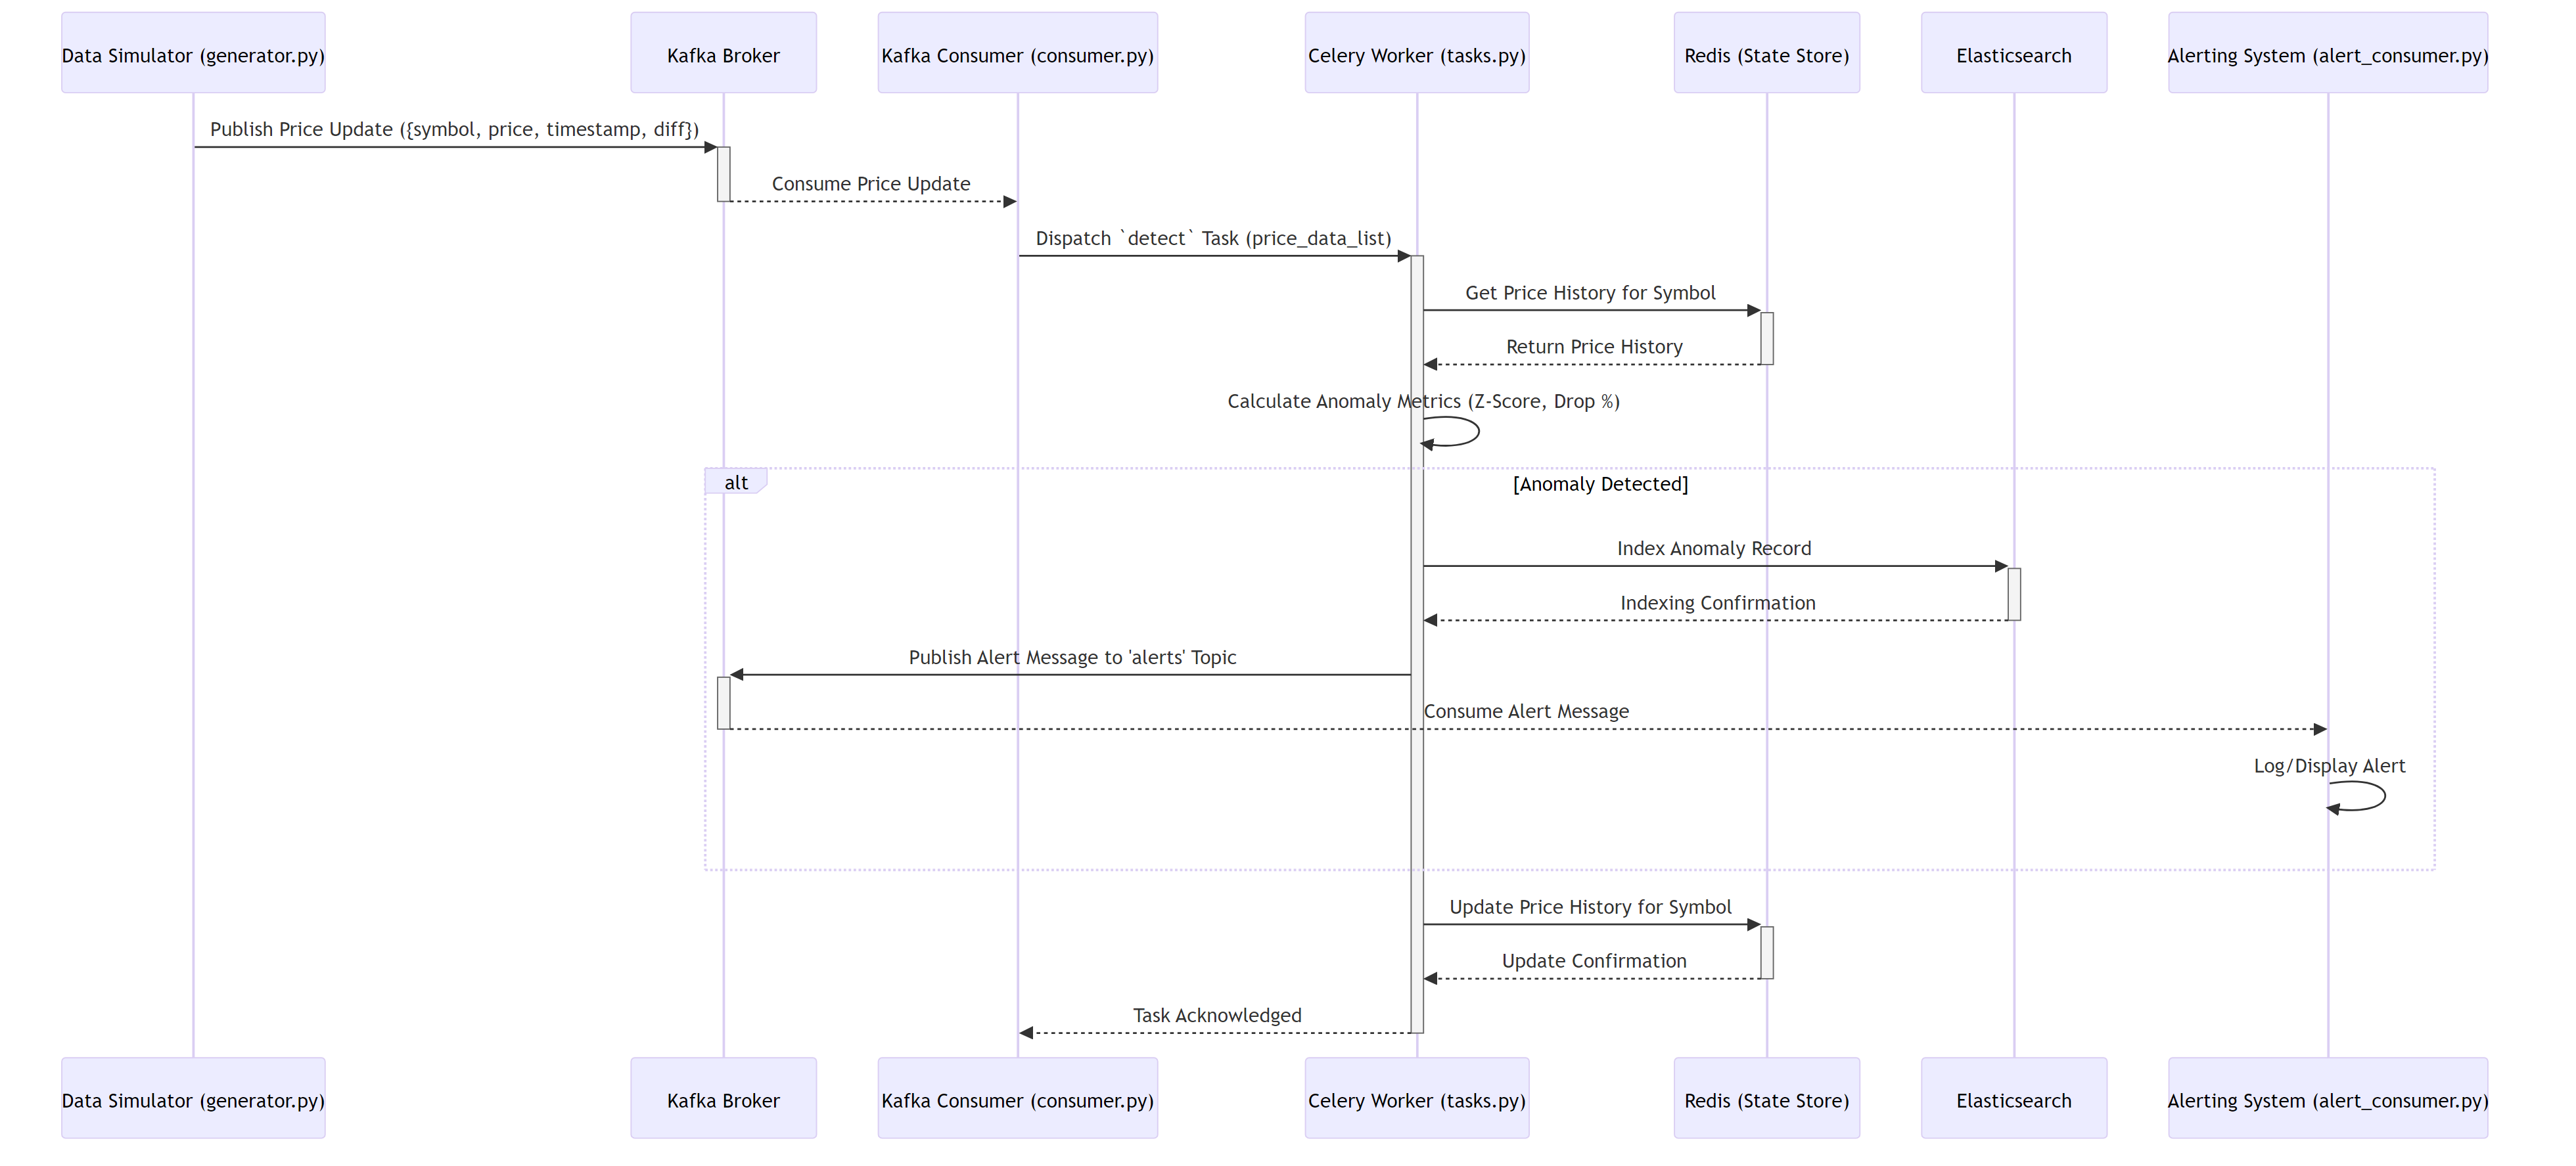
\includegraphics[width=\textwidth]{figures/backend-1.png}

\caption{A diagram showing the data flow for all the detail components described above,}

\label{fig:Expdiagram1}
\end{sidewaysfigure}

\break





\subsection{API and Reporting Layer}

\subsubsection{API Endpoints}
The Stock Anomaly Detection API provides several endpoints to fetch anomaly data and generate reports.

\paragraph{Alerting Endpoints}
\begin{itemize}
    \item \verb|GET /|: The root endpoint. Returns basic information about the API, including its name, version, and a list of available primary endpoints.
    \item \verb|GET /alerts|: Fetches all detected stock anomalies within a specified date range.
    \begin{itemize}
        \item Parameters: \verb|from| (start date), \verb|to| (end date).
    \end{itemize}
    \item \verb|GET /alerts/{symbol}/|: Retrieves anomalies for a specific stock symbol within a given date range.
    \begin{itemize}
        \item Parameters: \verb|symbol| (stock symbol), \verb|from| (start date), \verb|to| (end date).
    \end{itemize}
\end{itemize}

\paragraph{V1 Report Generation Endpoints}
The API offers robust report generation capabilities through its modern V1 endpoints, featuring powerful asynchronous operations.

\begin{itemize}
    \item \verb|POST /v1/reports|: This is the \textbf{primary endpoint} for all report-related operations. It offers a unified interface for both synchronous report generation and asynchronous generation with email delivery.
    \begin{itemize}
        \item Parameters: \verb|from|, \verb|to|, \verb|symbol|, \verb|format|.
        \item Optional Parameter: \verb|recipient_email|.
        \item \textbf{Behavior}:
        \begin{itemize}
            \item If \verb|recipient_email| is \textbf{not provided}, the report is generated synchronously and returned directly in the HTTP response.
            \item If \verb|recipient_email| \textbf{is provided}, the API gloriously initiates an \textbf{asynchronous background task} to generate the report. Upon successful completion, the report is automatically dispatched to the specified email address. This non-blocking operation allows users to continue interacting with other services or receive a quick acknowledgment (task ID) without waiting for the potentially time-consuming report generation process to finish.
        \end{itemize}
    \end{itemize}
    \item \verb|GET /v1/reports/status/{task_id}|: Allows users to check the status of an asynchronously initiated report generation task using the task ID returned by the \verb|/v1/reports| endpoint (when \verb|recipient_email| is used).
    \begin{itemize}
        \item Parameter: \verb|task_id|.
    \end{itemize}
\end{itemize}

The \verb|/v1/reports| endpoint significantly enhances user experience by providing a single, powerful interface for report generation. The asynchronous execution, particularly when coupled with email notifications, ensures that the system remains responsive and efficient, especially for large reports or during peak load times.




This next sequence diagram illustrates the interaction between the FastAPI application and the underlying data storage (Elasticsearch) and processing (Celery) for querying anomalies and generating reports.


% \subsection{Sequence Diagram: Api }

\begin{figure}[H]
    \centering
    % Placeholder for Class Diagram
    % \hspace{-3cm}
    % \includegraphics[width=0.8\textwidth]{figures/class_diagram_data_model.png}
    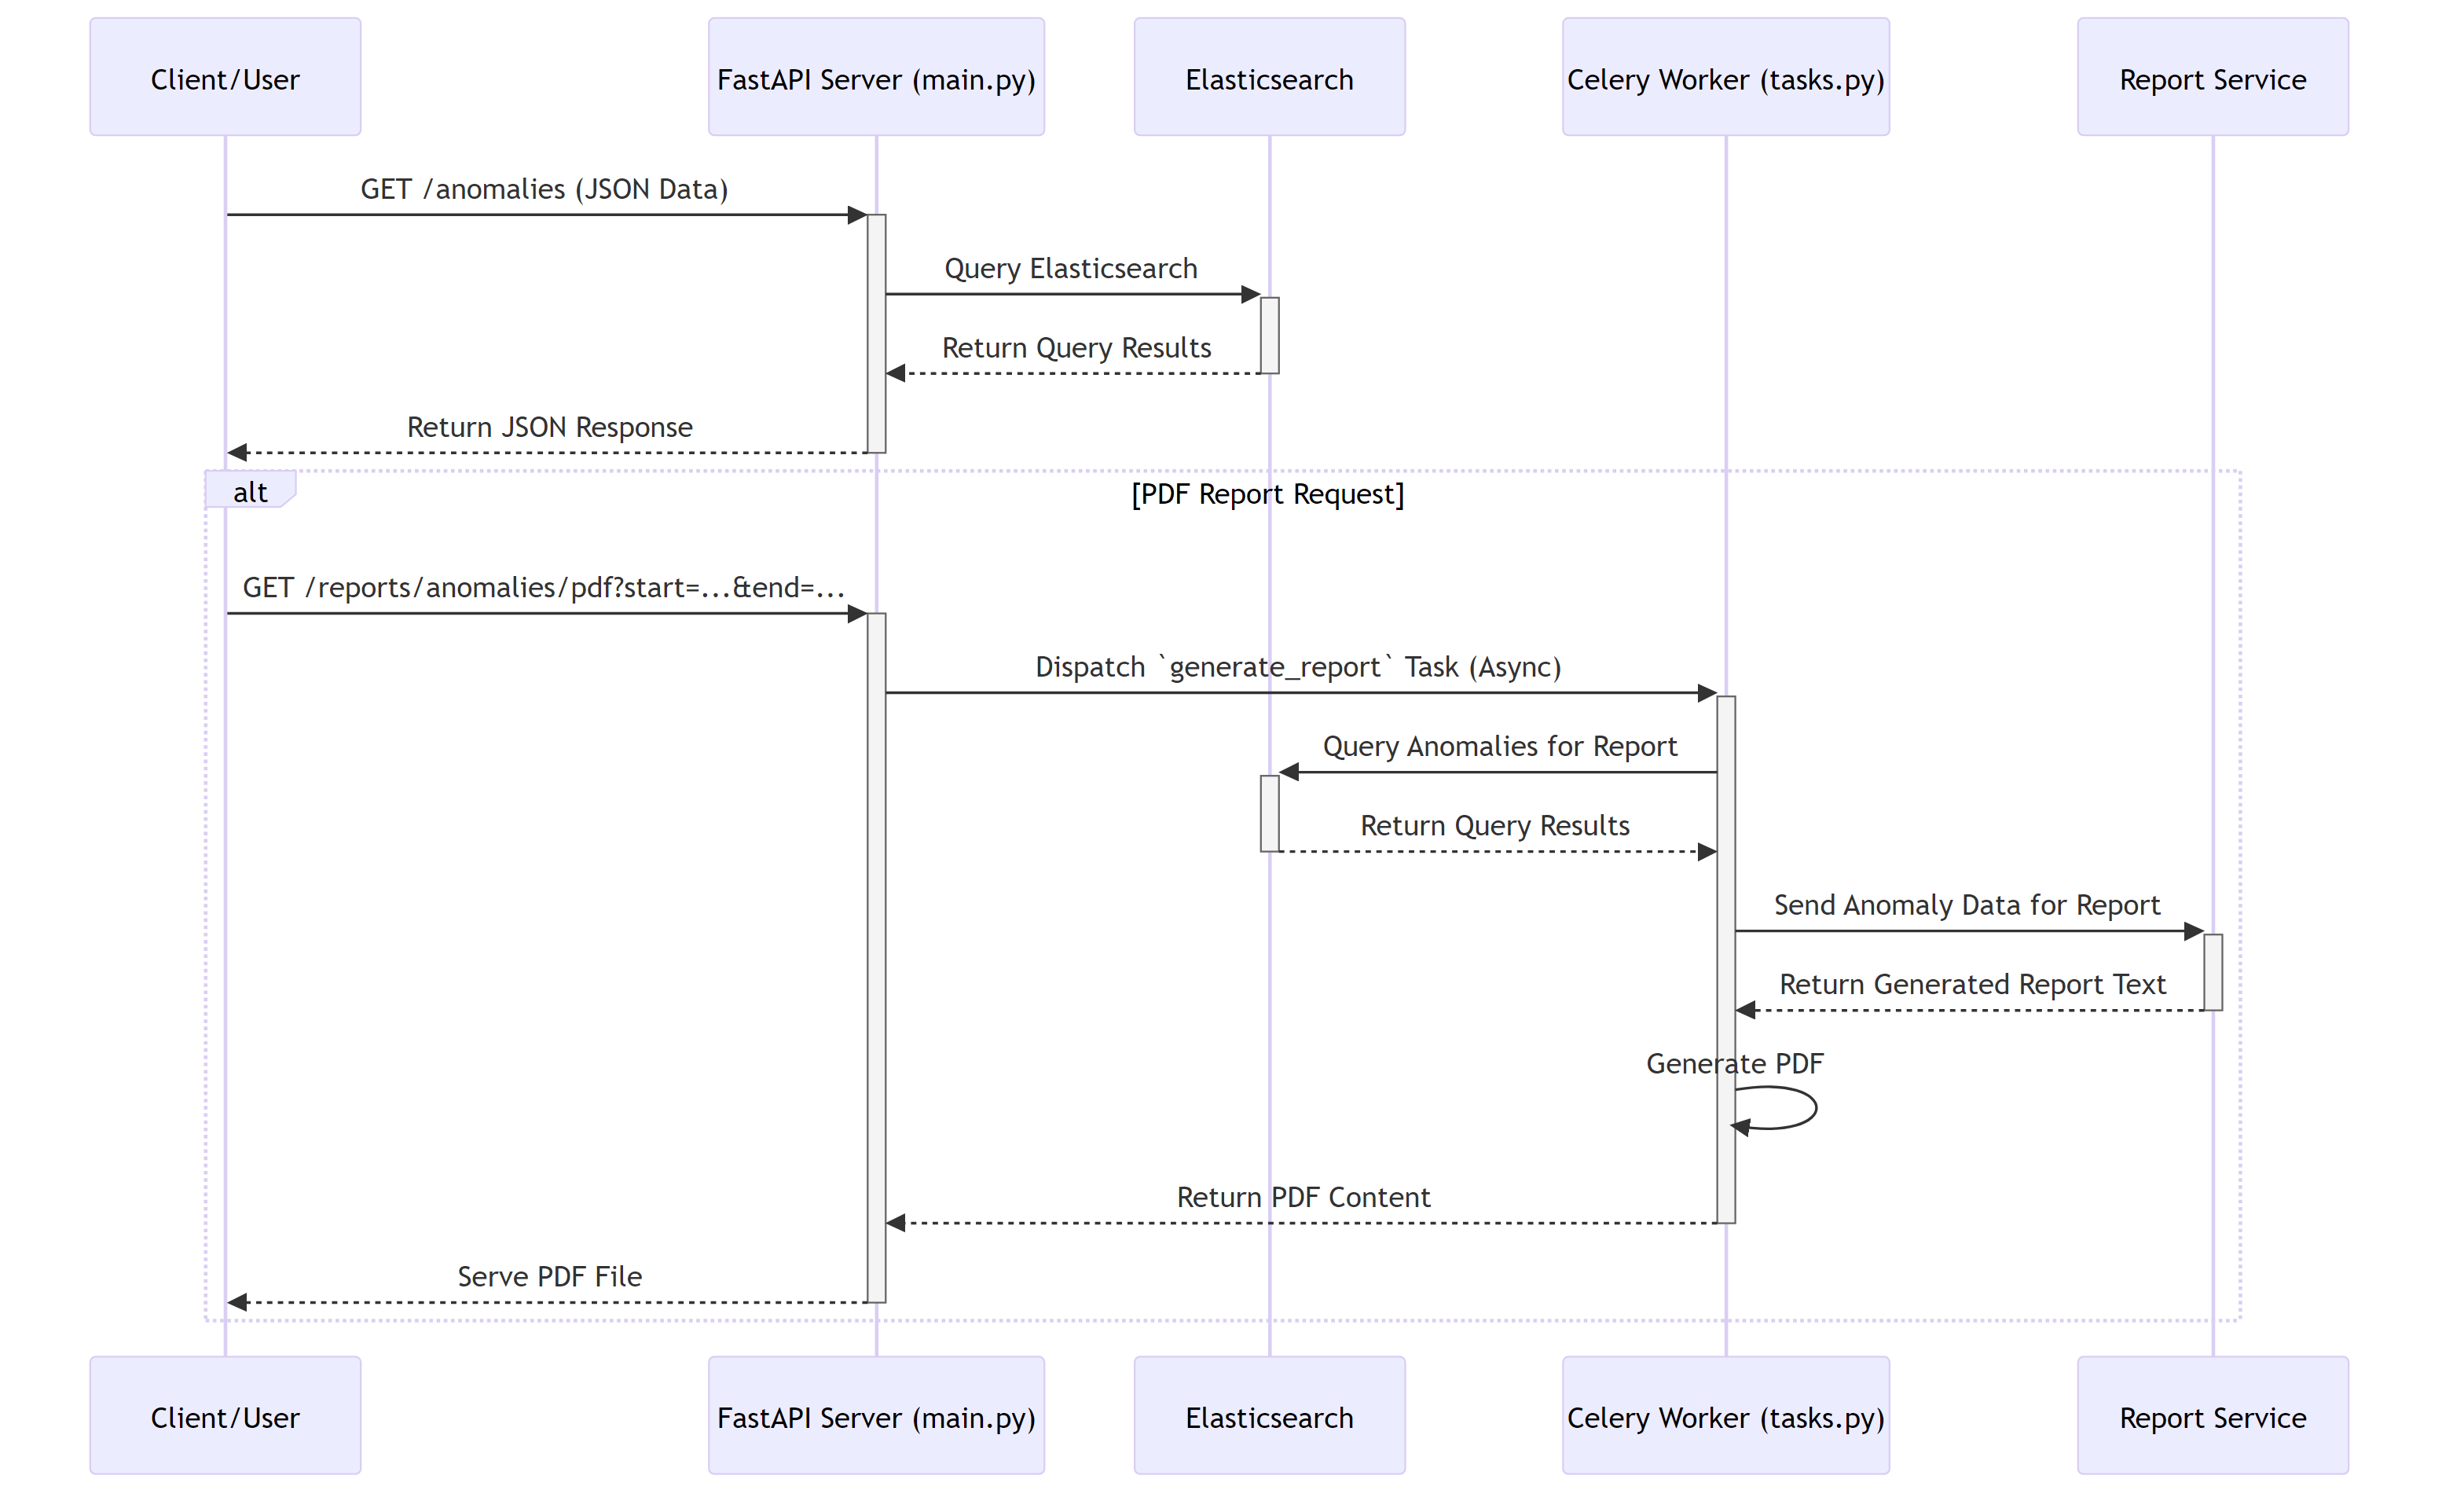
\includegraphics[width=1.2\textwidth,angle=90]{figures/api-1.png}
    \caption{Sequence Diagram for API Interactions}
    \label{fig:class_diagram_data_model}
\end{figure}

% This diagram would illustrate the sequence of interactions: FastAPI API $\rightarrow$ Elasticsearch (query anomalies) $\rightarrow$ Celery Worker (generate report) $\rightarrow$ FastAPI API (return report).
% it shows variant type of requests (geting anomalies, generating reports, etc.) and their interactions with the underlying data storage (Elasticsearch) and processing (Celery).



\subsubsection{Report Generator}

This module generates reports in multiple formats (PDF , CSV.....)
\begin{itemize}
    \item \textbf{Libraries}: `reportlab` for PDF.
    \item \textbf{Content}: Reports include summaries of detected anomalies, statistics, and potentially charts.
    \item \textbf{Formatting}: The formatting of the report depends on the selected format. For example, PDF reports can include sophisticated formatting with tables , enhancing readability and visual appeal. 

\begin{figure}[H]
    \centering
    \includegraphics[width=\textwidth]{figures/sad/pdf_screen.png}
    \caption{Sample PDF Report}
    \label{fig:pdf_report_screenshot}
\end{figure}

In contrast, CSV reports are formatted as comma-separated values, suitable for importing into spreadsheet software or other data analysis tools. 

\begin{figure}[H]
    \centering
    \includegraphics[width=\textwidth]{figures/sad/csv_screnn.png}
    \caption{Sample CSV Report}
    \label{fig:csv_report_screenshot}
\end{figure}
\end{itemize}

for the report generation, we use a Factory design pattern to create different report generators based on the requested format. This allows for easy extensibility if new report formats are needed in the future.
\subsection{Factory Pattern Diagram}
This diagram will illustrate the implementation of the Factory design pattern within the system, particularly for the data generation and anomaly detection modules. It will show the creator, concrete creators, product, and concrete product classes involved in the pattern.

This architecture utilizes the Factory Method design pattern, which provides an interface for creating objects in a superclass, but allows subclasses to alter the type of objects that will be created. In this specific context, the \texttt{ReportFactory} acts as the creator, abstracting the instantiation logic of different report generators (e.g., \texttt{PDFReportGenerator}, \texttt{CSVReportGenerator}).

\textbf{Why this pattern was used:}

The Factory Method pattern was chosen to decouple the client code from the concrete implementations of report generators. This means that the part of the application that needs a report doesn't need to know whether it's getting a PDF, CSV, or any other type of report. It simply requests a report generator from the \texttt{ReportFactory} based on a specified format. This promotes a clean separation of concerns and reduces direct dependencies.

\textbf{Scalability:}

This pattern significantly enhances scalability. If a new report format (e.g., Excel, XML) is required in the future, a new concrete \texttt{IReportGenerator} implementation (e.g., \texttt{ExcelReportGenerator}) can be added without modifying existing client code or the \texttt{ReportFactory}'s \texttt{get\_generator} method.

\begin{figure}[H]
    \centering
    % Placeholder for Class Diagram
    % \hspace{-3cm}
    % \includegraphics[width=0.8\textwidth]{figures/class_diagram_data_model.png}
    \includegraphics[width=\textwidth]{figures/generator-1.png}
    \caption{Factory Pattern Diagram}
    \label{fig:factory_pattern_diagram}
\end{figure}
 




\subsubsection{Alert System (Kafka Topics)}

When an anomaly is detected and confirmed, an alert message is published to a dedicated Kafka topic (e.g., \texttt{anomaly\_alerts}).
\begin{itemize}
    \item \textbf{Alert Message Format}: JSON, containing details of the anomaly and severity.
    \item \textbf{Consumers}: Separate services (not part of this core project scope but envisioned) can consume these alerts to send notifications via email, SMS, or dashboard updates.
\end{itemize}
\section{Justified Technology Choices}

\begin{itemize}
    \item \textbf{Apache Kafka}: Chosen for its high-throughput, fault-tolerant, and scalable stream processing capabilities, essential for handling real-time financial data feeds.
    
    \item \textbf{Elasticsearch}: Selected for its powerful full-text search, analytics capabilities, and horizontal scalability, making it ideal for storing, querying, and analyzing large volumes of anomaly data.
    
    \item \textbf{FastAPI (Python)}: Chosen for its high performance (comparable to NodeJS and Go), ease of use, automatic data validation with Pydantic, and built-in support for asynchronous programming, which is crucial for I/O-bound operations.
    
    \item \textbf{Celery (Python)}: Selected for distributed task processing. It allows decoupling time-consuming anomaly detection tasks from the main data ingestion flow, improving responsiveness and scalability.
    
    \item \textbf{Redis}: Chosen for its speed as an in-memory data store, perfect for managing sliding windows of recent price data required for Z-score calculations with minimal latency.
    
    \item \textbf{Python}: Used as the primary programming language due to its extensive libraries for data science (NumPy, Pandas), web development (FastAPI, Celery), and general-purpose programming, along with a large developer community.
    
    \item \textbf{Docker}: Used for containerization, ensuring consistent development, testing, and deployment environments across different machines and simplifying the management of microservices.
\end{itemize}

\section{Batch Report Generation and Deployment}








\subsection{sequence Diagram: Batch report generation}
\begin{figure}[H]
    
    % Placeholder for Class Diagram
    % \hspace{-3cm}
    % \includegraphics[width=0.8\textwidth]{figures/class_diagram_data_model.png}
    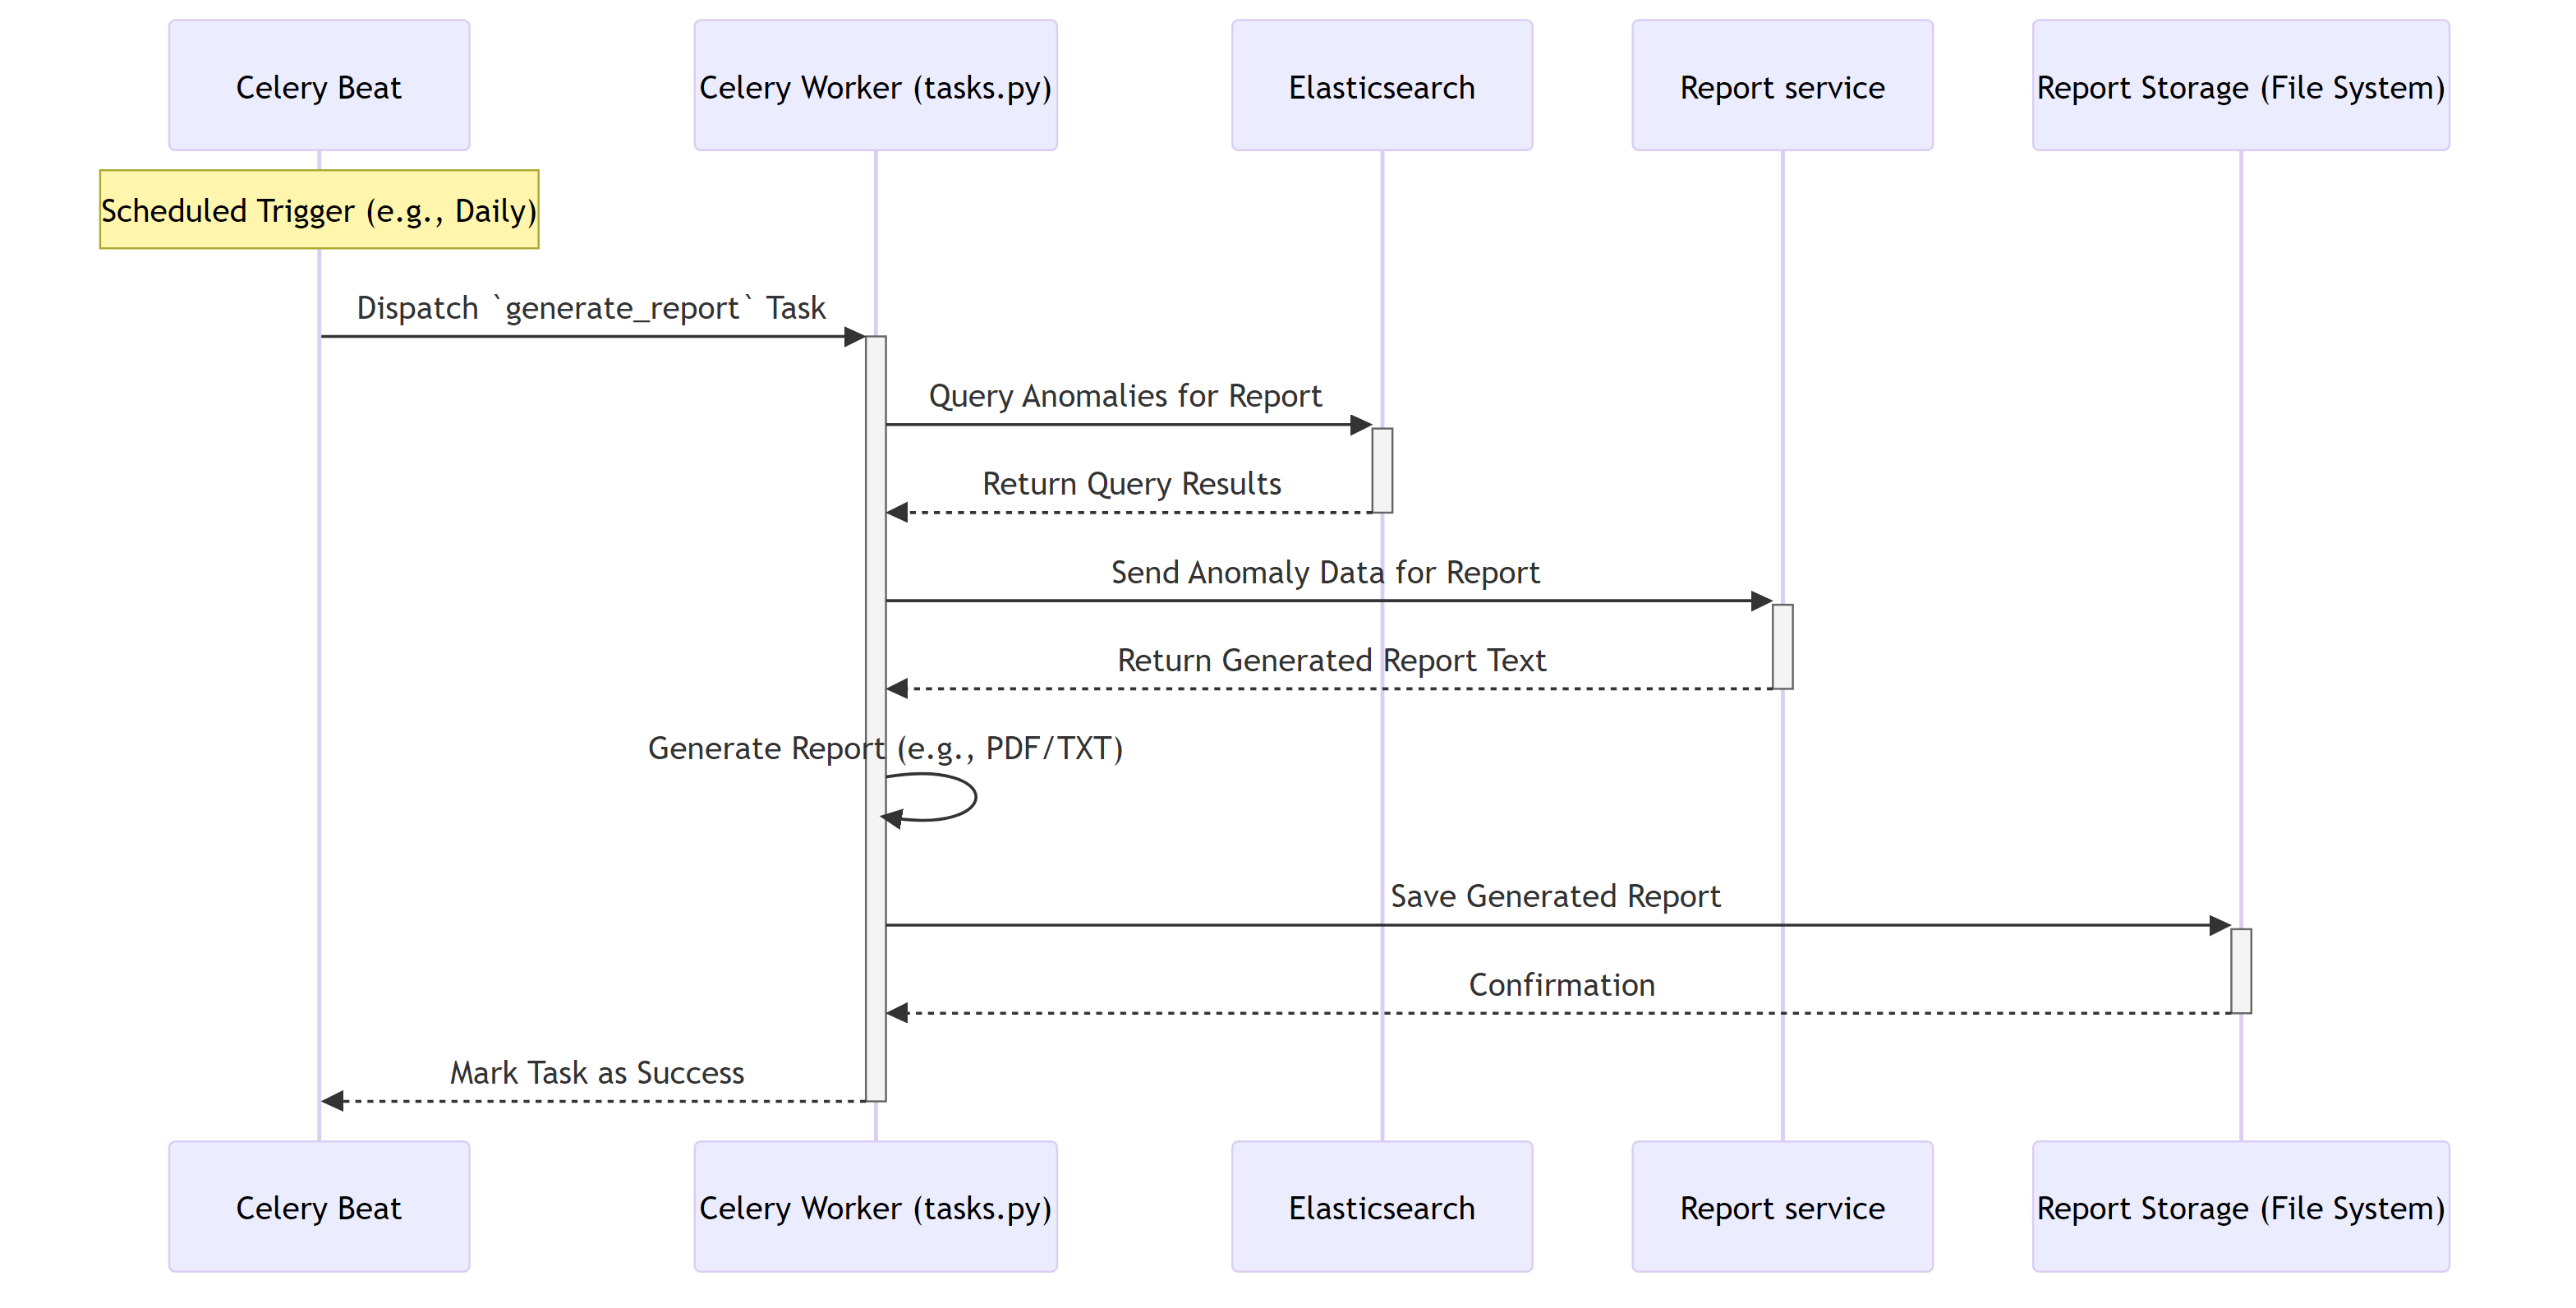
\includegraphics[width=1.2\textwidth]{figures/batch-1.png}
    \caption{Batch Report Generation Sequence Diagram}
    \label{fig:batch_report_generation_sequence_diagram}


\end{figure}


this diagram illustrate how shecduled batch report generation works, showing the interaction between the FastAPI application, Celery workers, and Elasticsearch for generating reports based on historical anomalies.
the layer responsibble for trigering the Task is the Celery Beat, which schedules the task to run at specific intervals (e.g., daily, weekly).
they work based on the linux cron system, which allows for scheduling tasks to run at specific times or intervals.

\subsection{Deployment with Docker and Docker Compose}

To orchestrate and run all the services in our architecture—Kafka, Zookeeper, Redis, Elasticsearch, and Kibana—we use Docker and Docker Compose. Docker allows us to package each service into a container, ensuring consistency across development, testing, and production environments.

\textbf{Service Ports and Networking:}
\begin{itemize}
    \item \textbf{Kafka} runs on port \texttt{9092} (for external connections) and \texttt{9093} (for internal container-to-container communication). These ports are mapped from the container to the host, allowing both local development tools and other containers to communicate with Kafka.
    \item \textbf{Zookeeper} (required by Kafka) listens on port \texttt{2181}.
    \item \textbf{Redis} runs on port \texttt{6379}. We use the \texttt{redis:7.2-alpine} image, which is based on Alpine Linux. Alpine images are chosen for their minimal size and security, reducing the attack surface and speeding up container startup.
    \item \textbf{Elasticsearch} is exposed on port \texttt{9200} for REST API access.
    \item \textbf{Kibana} is available on port \texttt{5601} for web-based visualization.
\end{itemize}

All containers are connected to a \textbf{shared Docker network} created by Docker Compose. This enables DNS-based service discovery: containers can communicate using service names (e.g., \texttt{kafka}, \texttt{redis}, \texttt{es01}) instead of IP addresses.

Docker Compose brought significant advantages to our deployment process by allowing us to define, configure, and launch all required services with a single command. It simplified service orchestration, ensured consistent environments, and made it easy to manage dependencies and networking between containers.

\begin{figure}[H]
    \centering
    \includegraphics[width=\textwidth]{figures/sad/image.png}
    \caption{Overall Docker Compose Architecture}
    \label{fig:docker_compose_architecture}
\end{figure}


This approach ensures that all services are reproducibly deployed, easily managed, and networked together, forming a robust foundation for our distributed financial data surveillance system.

% \subsection{Other UML Diagrams}
% This section provides placeholders for additional UML diagrams that can further illustrate the system's design. These diagrams will be added as the project evolves and specific design aspects require more detailed visualization.

% \subsubsection{Use Case Diagram}
% \begin{figure}[h]
%     \centering
%     \fbox{\parbox[c][6cm][c]{0.8\textwidth}{\centering Placeholder for Use Case Diagram}}
%     \caption{Placeholder for Use Case Diagram}
%     \label{fig:placeholder_use_case_diagram}
% \end{figure}

% \subsubsection{Component Diagram}
% \begin{figure}[h]
%     \centering
%     \fbox{\parbox[c][6cm][c]{0.8\textwidth}{\centering Placeholder for Component Diagram}}
%     \caption{Placeholder for Component Diagram}
%     \label{fig:placeholder_component_diagram}
% \end{figure}

% \subsubsection{Activity Diagram}
% \begin{figure}[h]
%     \centering
%     \fbox{\parbox[c][6cm][c]{0.8\textwidth}{\centering Placeholder for Activity Diagram}}
%     \caption{Placeholder for Activity Diagram}
%     \label{fig:placeholder_activity_diagram}
% \end{figure}

